\chapter{Introduction}
 
Nowadays, an ARM-MCU could be used in every aspect of everyday life.
Additionally, the ARM processor is the number one architecture of choice in 
many market segments.\\\\ 
This project is based on the development of a bootloaders and its implementation 
inside a network.The usage stm32f4-discovery Board is a prefered and viewed as an 
"'Allrounder"' for such a project. The reasoning behind this is the "value for money" 
and user-friendliness. This allows for an easy introduction into the world of ARM
Microcontroller unit programming.\\
The ARM-Cortex-M4-Prozessor found on the STM32f4-discovery board processes 
the principel parts shown in the figure below.\\
The aim of the project is to research the feasibility to create a quick, cheap 
and easy to use way of utilizing an STM32 Microcontroller to communicate between 
a user and a remote device.\\\\
The purpose of the application is meant to be a first step fundamental strategy to 
creating a product for future projects.\\
It is hoped that by utilizing a boot loader, a fast and light application could 
be used to fulfill the desire of a user to achieve a particular objective such 
as, threeway handshake signal to verify a particular device in order to transmit 
information such as codes or messages, using a TCP/IP protocol stake.\\
As it can be demonstrated the different applications could be endless.\\ 

\begin{figure}[ht]
	\centering
	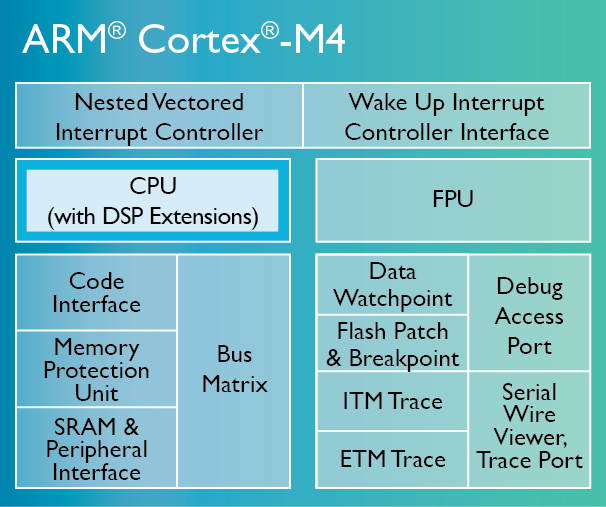
\includegraphics[width=400px, height=300px]{../img/Cortex-M4-chip-diagram-LG.png}
	\caption{Prinzipieller Aufbau}
	\label{m4_prinzip}
\end{figure}

Analogously, a new and different diagram would be used, in order to illustrate the 
change in the usage-concept of the processors.\\

But first, an overview of the discussed focal points would be outlined.\\  


\section{Bootloader}
The purpose of a Bootloader program is to allow the installation and utilisation 
of any program that could be reloaded. Whereas the program that is currently loaded is also being run.\\
Next it is necessary to initialise the hardware, that would in turn be needed to load the program.\\
The "STM32f407 discovery board" offers three different methodes to boot up the hardware.\\
In order to switch between the three different boot methods, the Boot-Pins BOOT1
and BOOT2 could be set:
\begin{table}[ht]
\caption{Boot-Pin Function}
\begin{tabular}{|c|c|l|l|}
\hline \hline
  BOOT1 & BOOT2 & Boot-Mode & Adresse\\ \hline
  x & 0 & Flash Memory (User Flash) & 0x8000\_0000\\
\hline
  0 & 1 & System Memory & 0x1FFF\_F000\\
\hline
 1  & 1 & SRAM & 0x2000\_0000\\
\hline
\end{tabular}
\end{table}\\\\

The ROM memory is included by the manufacturer along with the bootloader.\\
It is very important to set the correct address of the program, that is located 
in the memory, in order for the reloading of the program to work.\\
A step by step example of the the sequence after the boot loader is already 
loaded , is as follows:

\begin{enumerate}
\item Hardware initialize (USB / USART / RCC ... )
\item Wait for running program (pending other tasks)
\item Write a program to address XY.
\item Point to address XY
\end{enumerate}

After these steps, the newly setup program is then responsible for the initialization 
of the hardware.\\

\section{SWD}
During the development of the Boot Loader, a the serial wire debug technology was used. 
The reason behind this is to utilize a Debug-Port that has been specially developed to 
cater to a MCU that makes allows the use of the least amount of pins possible.\\
This port consists of pins shown in the following:\\\\
\begin{table}
\caption{SWD PINOUT}
\begin{tabular}{|c|c|c|p{10cm}|}
\hline \hline
	Pin & Signal & Type & Description \\ \hline
1 & VTref & Input & This is the target reference voltage. It is used to
 check if the target has power, to create the logic-level reference for
 the input comparators and to control the output logic levels to the target.
 It is normally fed from Vdd of the target board and must not have a series resistor.\\ \hline
7 & SWDIO & I/O & Single bi-directional data pin\\ \hline
9 & SWCLK & Output & Clock signal to target CPU. It is recommended that
 this pin is pulled to a defined state of the target board. Typically
 connected to TCK of target CPU.\\ \hline
13 & SWO & Output & Serial Wire Output trace port. (Optional, not required
for SWD communication)\\ \hline
15 & RESET & I/O & Target CPU reset signal. Typically connected to the
 RESET pin of the target CPU, which is typically called "nRST", "nRESET"
 or "RESET".\\ \hline
19 & 5V-Supply & Output & This pin is used to supply power to some eval boards.
Not all JLinks supply power on this pin, only the KS (Kickstart) versions.
Typically left open on target hardware.\\ \hline
\end{tabular}
\end{table}\\\\

The other pins of the 20-pole connection are going to left out, meaning, the other 
pins are useless for the SWD or they will be used as a GND. Regardless of the pin allocation, 
it is important that the communication of the SWD would not be interrupted or effected. 

This technique represents a new and more effective way to debuggen. Until now JTAG 
represented the Debugger-Interface.  

Die Vorteile dieser Technologie sind (frei von der ARM-Website \"ubersetzt):

\begin{itemize}
\item Only 2 Pins are used
\item JTAG TAP controller compatible
\item Allows the Debugger to become an extra AMBA-Bus-Master, in order to accomidate an extra 
access capability to the Register or Memory
\item High Datarates - 4Mbytes/sec @50MHz
\item Low Power - no extra power supply 
\item Error recognition "'built in"' that performs well
\item Protection against errors that cause disconnection
\end{itemize}  

\section{startup}
 - stack, program counter, interrupt, vector table, initial system clock

\section{CMSIS}
The ARM Cortex Microcontroller Software Interface Standard is a manufacturer independent 
abstraction layer for the Cortex-M processors.\\
Thereby the CMSIS is subdivided into:
\begin{itemize}
\item CMSIS-CORE - API access to the processor kernal and peripheral register.
\item CMSIS-Driver - Generic access on peripheral devices for Middleware
			(reusability).
\item CMSIS-DSP - DSP Liberary with over 60 functions
\item CMSIS-RTOS API - Standardised (RTOS compatible)
\item CMSIS-Pack - Description of the most important components (User view)
\item CMSIS-SVD - Description of the most important components (System view)
\item CMSIS-DAP - Debug Access Port
\end{itemize}

Summarized, CMSIS allows a consistent and simple software interfaced to the processor 
and peripheral devices, as well as Real-time OS (RTOS) and Middleware.

\section{Nested Vectored Interrupt Controller}
The NVIC offers the possibility to configure special interrupts 
(Priority, Activate, Deactivate...). \\
Aside from the given Interrupts, there are also the configurable implementation dependent interrupts.  
Because, the first 15 interrupts are allocated, the number of implimented interrupts could be from 0-240.

\section{Differences }
GNU, KEIL iar

\section{Network}
was sollte zum besseren verstehen hier einen platz finden.
